         \chapter{The Hydrosphere}\fancyfoot[LO,RE]{Chemistry: Chemical systems}
    \setcounter{figure}{1}
    \setcounter{subfigure}{1}
    \label{m38138}
    \section{Introduction}
            \nopagebreak
            \label{m38138*cid2} $ \hspace{-5pt}\begin{array}{cccccccccccc}   \end{array} $ \hspace{2 pt}\raisebox{-5 pt}{
\includegraphics[width=0.5cm]{col11305.imgs/summary_www.png}} {(section shortcode: P10107 )} \par 
\begin{minipage}{.7\textwidth}
      \label{m38138*id334056}As far as we know, the Earth we live on is the only planet that is able to support life. Amongst other factors, the Earth is just the right distance from the sun to have temperatures that are suitable for life to exist. Also, the Earth's atmosphere has exactly the right type of gases in the right amounts for life to survive. Our planet also has \textbf{water} on its surface, which is something very unique. In fact, Earth is often called the 'Blue Planet' because most of it is covered in water. This water is made up of \textsl{freshwater} in rivers and lakes, the \textsl{saltwater} of the oceans and estuaries, \textsl{groundwater} and \textsl{water vapour}. Together, all these water bodies are called the \textbf{hydrosphere}.\par 
\end{minipage}
\begin{minipage}{.3\textwidth}
\begin{center}
 \includegraphics[width=0.6\textwidth]{photos/earth_space_nasa-flickr.jpg}\\
\textsl{Photo by NASA on flickr}
\end{center}

\end{minipage}

      \label{m38138*id8754}
\begin{tabular}{cc}
	\hspace*{-50pt}\raisebox{-8 mm}{\hspace{-0.2in}
\includegraphics[width=0.75in]{col11305.imgs/psfact2.png} } & 
	\begin{minipage}{0.85\textwidth}
	\begin{note}
      {note: }The total mass of the hydrosphere is approximately $1,4\ensuremath{\times}{10}^{18}\phantom{\rule{2pt}{0ex}}\mathrm{tonnes}$! (The volume of one tonne of water is approximately 1 cubic metre.)
	\end{note}
	\end{minipage}
	\end{tabular}
	\par
    \section{Interactions of the hydrosphere}
            \nopagebreak
            \label{m38138*cid3} $ \hspace{-5pt}\begin{array}{cccccccccccc}   \end{array} $ \hspace{2 pt}\raisebox{-5 pt}{
\includegraphics[width=0.5cm]{col11305.imgs/summary_www.png}} {(section shortcode: P10108 )} \par 
      \label{m38138*id334443}It is important to realise that the hydrosphere is not an isolated system, but rather interacts with other global systems, including the \textsl{atmosphere}, \textsl{lithosphere} and \textsl{biosphere}. These interactions are sometimes known collectively as the water cycle.\par 

      \label{m38138*id334463}\begin{itemize}[noitemsep]
            \label{m38138*uid1}\item \textsl{Atmosphere}
When water is heated (e.g. by energy from the sun), it evaporates and forms water vapour. When water vapour cools again, it condenses to form liquid water which eventually returns to the surface by precipitation e.g. rain or snow. This cycle of water moving through the atmosphere and the energy changes that accompany it, is what drives weather patterns on earth.
\label{m38138*uid2}\item \textsl{Lithosphere} \\
\begin{minipage}{.6\textwidth}
In the lithosphere (the ocean and continental crust at the Earth's surface), water is an important \textsl{weathering} agent, which means that it helps to break rock down into rock fragments and then soil. These fragments may then be transported by water to another place, where they are deposited. These two processes (weathering and the transporting of fragments) are collectively called \textsl{erosion}. Erosion helps to shape the earth's surface. For example, you can see this in rivers. In the upper streams, rocks are eroded and sediments are transported down the river and deposited on the wide flood plains lower down. On a bigger scale, river valleys in mountains have been carved out by the action of water, and cliffs and caves on rocky beach coastlines are also the result of weathering and erosion by water. The processes of weathering and erosion also increase the content of dissolved minerals in the water. These dissolved minerals are important for the plants and animals that live in the water.
\end{minipage}
\begin{minipage}{.4\textwidth}
 \begin{center}
  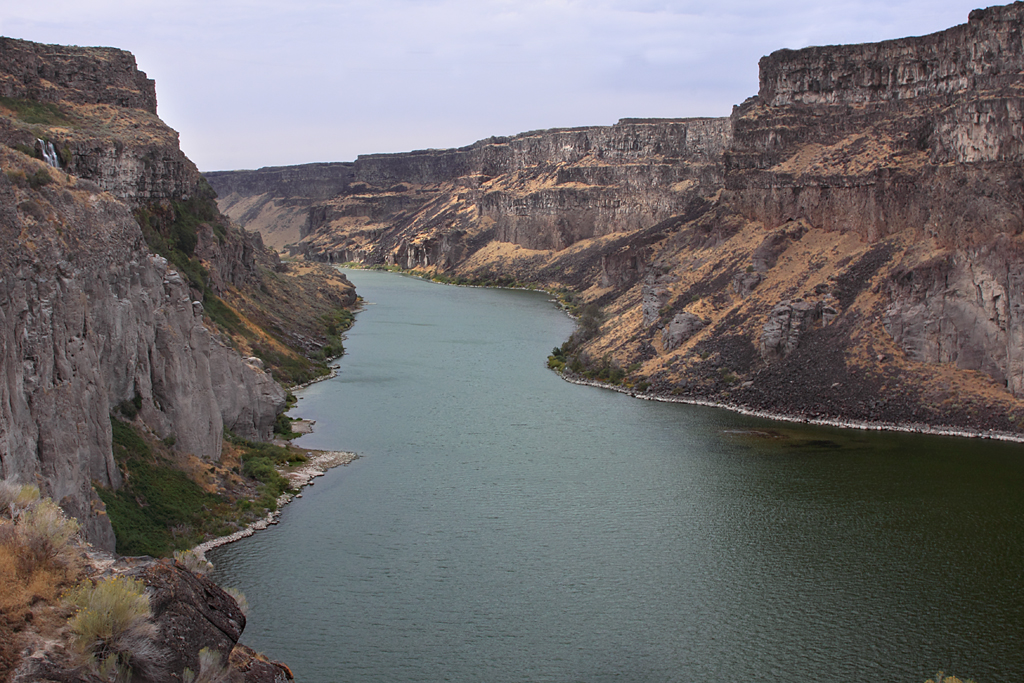
\includegraphics[width=.6\textwidth]{photos/AlanVernon.jpg}\\
\textsl{photo by AlanVernon on flickr}
 \end{center}
\end{minipage}
\label{m38138*uid3}\item \textsl{Biosphere}
In the biosphere, land plants absorb water through their roots and then transport this through their vascular (transport) system to stems and leaves. This water is needed in \textsl{photosynthesis}, the food production process in plants. Transpiration (evaporation of water from the leaf surface) then returns water back to the atmosphere.
\end{itemize}


    \section{Exploring the Hydrosphere}
            \nopagebreak
            \label{m38138*cid4} $ \hspace{-5pt}\begin{array}{cccccccccccc}   \end{array} $ \hspace{2 pt}\raisebox{-5 pt}{
\includegraphics[width=0.5cm]{col11305.imgs/summary_www.png}} {(section shortcode: P10109 )} \par 
      \label{m38138*id334557}The large amount of water on our planet is something quite unique. In fact, about 71\% of the earth is covered by water. Of this, almost 97\% is found in the oceans as saltwater, about 2.2\% occurs as a solid in ice sheets, while the remaining amount (less than 1\%) is available as freshwater. So from a human perspective, despite the vast amount of water on the planet, only a very small amount is actually available for human consumption (e.g. drinking water). In Reactions in aqueous solutions\footnote{\raggedright{}"Reactions in aqueous solutions - Grade 10 [CAPS]" <http://http://cnx.org/content/m38136/latest/>} we looked at some of the reactions that occur in aqueous solution and saw some of the chemistry of water, in this section we are going to spend some time exploring a part of the hydrosphere in order to start appreciating what a complex and beautiful part of the world it is. After completing the following investigation, you should start to see just how important it is to know about the chemistry of water.\par 
\label{m38138*secfhsst!!!underscore!!!id86}
            \begin{Investigation}{Investigating the hydrosphere
      }
            \nopagebreak 
\begin{minipage}{.5\textwidth}
            \label{m38138*uid4}
For this exercise, you can choose any part of the hydrosphere that you would like to explore. This may be a rock pool, a lake, river, wetland or even just a small pond. The guidelines below will apply best to a river investigation, but you can ask similar questions and gather similar data in other areas. When choosing your study site, consider how accessible it is (how easy is it to get to?) and the problems you may experience (e.g. tides, rain).\par
\label{m38138*uid5}
Your teacher will provide you with the equipment you need to collect the following data. You should have at least one study site where you will collect data, but you might decide to have more if you want to compare your results in different areas. This works best in a river, where you can choose sites down its length. \par
\end{minipage}
\begin{minipage}{.5\textwidth}
\begin{center}
 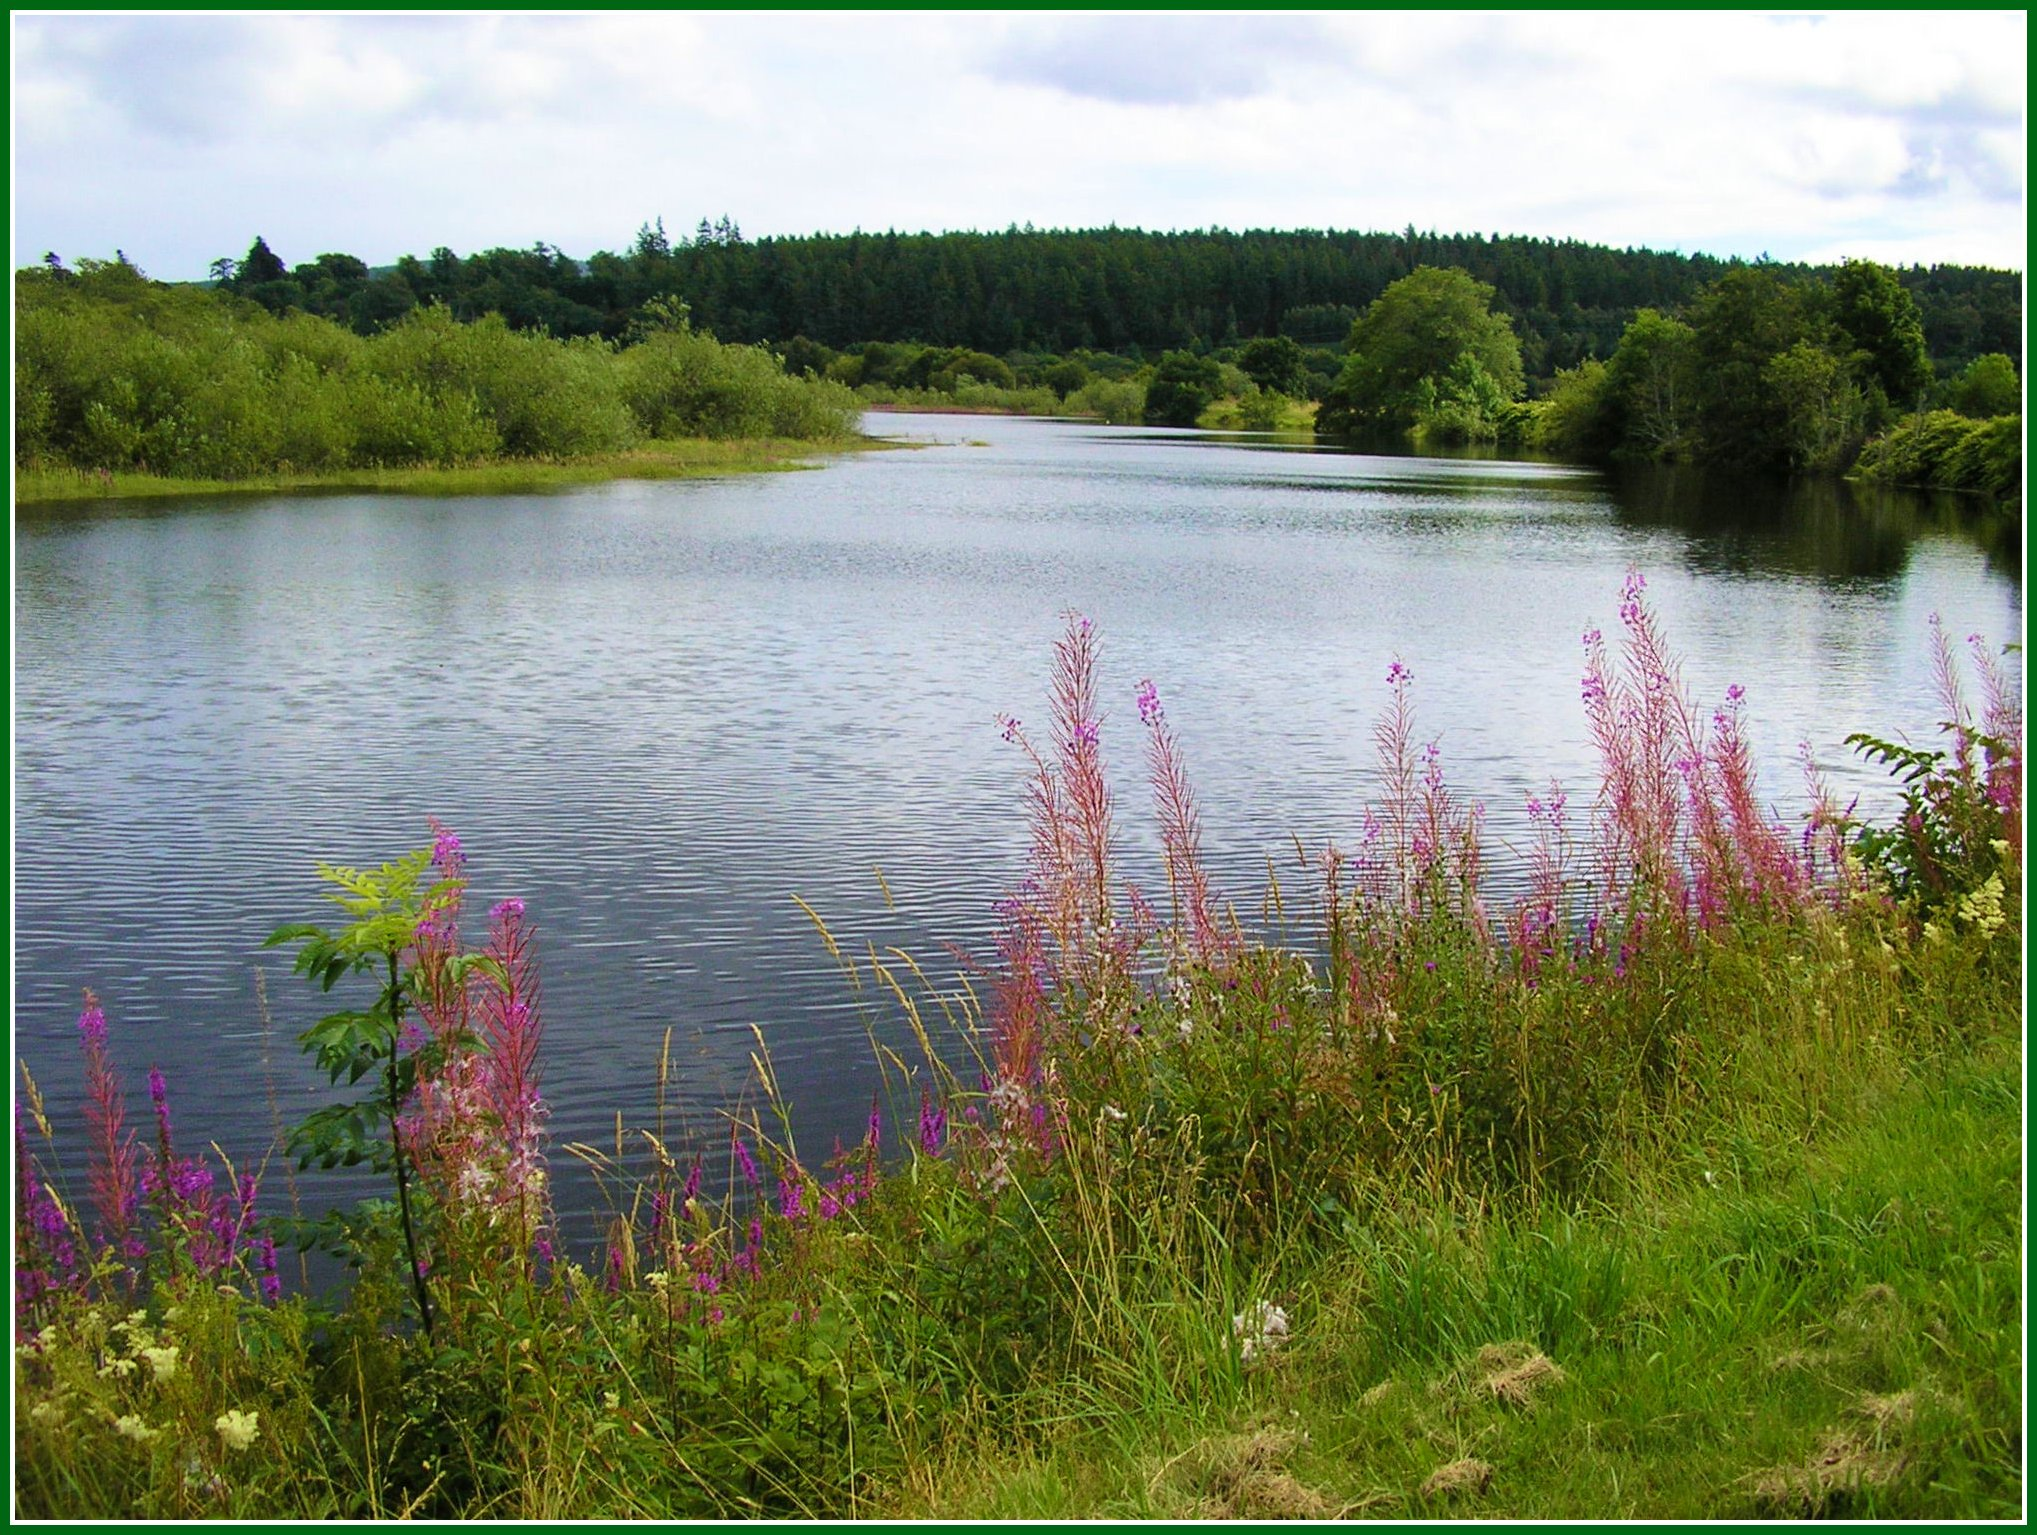
\includegraphics[width=.8\textwidth]{photos/DuncanBrown(Cradlehall).jpg} \\
\textsl{Photo by Duncan Brown (Cradlehall) on flickr}
\end{center}
\end{minipage}
\label{m38138*id334646}\begin{enumerate}[noitemsep, label=\textbf{\arabic*}. ] 
            \label{m38138*uid6}\item \textsl{Chemical data}
Measure and record data such as temperature, pH, conductivity and dissolved oxygen at each of your sites. You may not know exactly what these measurements mean right now, but it will become clearer later.
\label{m38138*uid7}\item \textsl{Hydrological data}
Measure the water velocity of the river and observe how the volume of water in the river changes as you move down its length. You can also collect a water sample in a clear bottle, hold it to the light and see whether the water is clear or whether it has particles in it.
\label{m38138*uid8}\item \textsl{Biological data}
What types of animals and plants are found in or near this part of the hydrosphere? Are they specially adapted to their environment?
\end{enumerate}

Record your data in a table like the one shown below:
    % \textbf{m38138*id334712}\par
          \begin{table}[H]
    % \begin{table}[H]
    % \\ 'id3029941' '1'
        \begin{center}
      \label{m38138*id334712}
    \noindent
    \tabletail{%
        \hline
        \multicolumn{4}{|p{\mytableboxwidth}|}{\raggedleft \small \sl continued on next page}\\
        \hline
      }
      \tablelasttail{}
      \begin{xtabular}[t]{|l|l|l|l|}\hline
         &
        \textbf{Site 1} &
        \textbf{Site 2} &
        \textbf{Site 3}% make-rowspan-placeholders
     \tabularnewline\cline{1-1}\cline{2-2}\cline{3-3}\cline{4-4}
      %--------------------------------------------------------------------
        \textbf{Temperature} &
         &
         &
        % make-rowspan-placeholders
     \tabularnewline\cline{1-1}\cline{2-2}\cline{3-3}\cline{4-4}
      %--------------------------------------------------------------------
        \textbf{pH} &
         &
         &
        % make-rowspan-placeholders
     \tabularnewline\cline{1-1}\cline{2-2}\cline{3-3}\cline{4-4}
      %--------------------------------------------------------------------
        \textbf{Conductivity} &
         &
         &
        % make-rowspan-placeholders
     \tabularnewline\cline{1-1}\cline{2-2}\cline{3-3}\cline{4-4}
      %--------------------------------------------------------------------
        \textbf{Dissolved oxygen} &
         &
         &
        % make-rowspan-placeholders
     \tabularnewline\cline{1-1}\cline{2-2}\cline{3-3}\cline{4-4}
      %--------------------------------------------------------------------
        \textbf{Animals and plants} &
         &
         &
        % make-rowspan-placeholders
     \tabularnewline\cline{1-1}\cline{2-2}\cline{3-3}\cline{4-4}
      %--------------------------------------------------------------------
    \end{xtabular}
      \end{center}
\end{table}
    \par
  \label{m38138*uid9}\item \textbf{Interpreting the data}
Once you have collected and recorded your data, think about the following questions:
\label{m38138*id334958}\begin{itemize}[noitemsep]
            \label{m38138*uid10}\item How does the data you have collected vary at different sites?
\label{m38138*uid11}\item Can you explain these differences?
\label{m38138*uid12}\item What effect do you think \textsl{temperature}, \textsl{dissolved oxygen} and \textsl{pH} have on animals and plants that are living in the hydrosphere?
\label{m38138*uid13}\item Water is seldom 'pure'. It usually has lots of things dissolved (e.g. ${Mg}^{2+}$, ${Ca}^{2+}$ and $\mathrm{NO}_{3}^{-}$ ions) or suspended (e.g. soil particles, debris) in it. Where do these substances come from?
\label{m38138*uid14}\item Are there any human activities near this part of the hydrosphere? What effect could these activities have on the hydrosphere?
\end{itemize}
\end{Investigation}
    \section{The Importance of the Hydrosphere}
            \nopagebreak
            \label{m38138*cid5} $ \hspace{-5pt}\begin{array}{cccccccccccc}   \end{array} $ \hspace{2 pt}\raisebox{-5 pt}{
\includegraphics[width=0.5cm]{col11305.imgs/summary_www.png}} {(section shortcode: P10110 )} \par 
      \label{m38138*id335077}It is so easy sometimes to take our hydrosphere for granted and we seldom take the time to really think about the role that this part of the planet plays in keeping us alive. Below are just some of the very important functions of water in the hydrosphere:\par 
      \label{m38138*id335082}\begin{itemize}[noitemsep]
            \label{m38138*uid15}\item \textsl{Water is a part of living cells}
Each cell in a living organism is made up of almost 75\% water, and this allows the cell to function normally. In fact, most of the chemical reactions that occur in life, involve substances that are dissolved in water. Without water, cells would not be able to carry out their normal functions and life could not exist.
\label{m38138*uid16}\item \textsl{Water provides a habitat}
The hydrosphere provides an important place for many animals and plants to live. Many gases (e.g. ${\mathrm{CO}}_{2}$, ${\mathrm{O}}_{2}$), nutrients e.g. nitrate ($\mathrm{NO}_{3}^{-}$), nitrite ($\mathrm{NO}_{2}^{-}$) and ammonium ($\mathrm{NH}_{4}^{+}$) ions, as well as other ions (e.g. ${Mg}^{2+}$ and ${Ca}^{2+}$) are dissolved in water. The presence of these substances is critical for life to exist in water.
\label{m38138*uid17}\item \textsl{Regulating climate}
One of water's unique characteristics is its high \textsl{specific heat}. This means that water takes a long time to heat up and also a long time to cool down. This is important in helping to regulate temperatures on earth so that they stay within a range that is acceptable for life to exist. \textsl{Ocean currents} also help to disperse heat.
\label{m38138*uid18}\item \textsl{Human needs}
Humans use water in a number of ways. Drinking water is obviously very important, but water is also used domestically (e.g. washing and cleaning) and in industry. Water can also be used to generate electricity through hydropower.
\end{itemize}
      \label{m38138*id335280}These are just a few of the very important functions that water plays on our planet. Many of the functions of water relate to its chemistry and to the way in which it is able to dissolve substances in it.\par 
    \section{Threats to the Hydrosphere}
            \nopagebreak
            \label{m38138*cid10} $ \hspace{-5pt}\begin{array}{cccccccccccc}   \end{array} $ \hspace{2 pt}\raisebox{-5 pt}{
\includegraphics[width=0.5cm]{col11305.imgs/summary_www.png}} {(section shortcode: P10111 )} \par 
      \label{m38138*id342204}It should be clear by now that the hydrosphere plays an extremely important role in the survival of life on Earth and that the unique properties of water allow various important chemical processes to take place which would otherwise not be possible. Unfortunately for us however, there are a number of factors that threaten our hydrosphere and most of these threats are because of human activities. We are going to focus on two of these issues: \textbf{overuse} and \textbf{pollution} and look at ways in which these problems can possibly be overcome.\par 
      \label{m38138*id342223}\begin{enumerate}[noitemsep, label=\textbf{\arabic*}. ] 
            \label{m38138*uid91}\item \textbf{Pollution}\newline
Pollution of the hydrosphere is also a major problem. When we think of pollution, we sometimes only think of things like plastic, bottles, oil and so on. But any chemical that is present in the hydrosphere in an amount that is not what it should be is a pollutant. Animals and plants that live in the Earth's water bodies are specially adapted to surviving within a certain range of conditions. If these conditions are changed (e.g. through pollution), these organisms may not be able to survive. Pollution then, can affect entire aquatic ecosystems. The most common forms of pollution in the hydrosphere are \textsl{waste products} from humans and from industries, \textsl{nutrient pollution} e.g. fertiliser runoff which causes eutrophication (an excess of nutrients in the water leading to excessive plant growth) and toxic trace elements such as aluminium, mercury and copper to name a few. Most of these elements come from mines or from industries.
\label{m38138*uid87}\item \textbf{Overuse of water}\newline
We mentioned earlier that only a very small percentage of the hydrosphere's water is available as freshwater. However, despite this, humans continue to use more and more water to the point where water \textsl{consumption} is fast approaching the amount of water that is \textsl{available}. The situation is a serious one, particularly in countries such as South Africa which are naturally dry and where water resources are limited. It is estimated that between 2020 and 2040, water supplies in South Africa will no longer be able to meet the growing demand for water in this country. This is partly due to population growth, but also because of the increasing needs of industries as they expand and develop. For each of us, this should be a very scary thought. Try to imagine a day without water... difficult isn't it? Water is so much a part of our lives, that we are hardly aware of the huge part that it plays in our daily lives.
\end{enumerate}
\label{m38138*secfhsst!!!underscore!!!id1046}
            \begin{groupdiscussion}{ Creative water conservation
}
            \nopagebreak

\label{m38138*uid289435}As populations grow, so do the demands that are placed on dwindling water resources. While many people argue that building dams helps to solve this water-shortage problem, there is evidence that dams are only a temporary solution and that they often end up doing far more ecological damage than good. The only sustainable solution is to reduce the \textsl{demand} for water, so that water supplies are sufficient to meet this. The more important question then is how to do this.
\par 
\label{m38138*uid5630}\textbf{Discussion:}\newline
\begin{minipage}{.6\textwidth}
    Divide the class into groups, so that there are about five people in each. Each group is going to represent a different sector within society. Your teacher will tell you which sector you belong to from the following: Farming, industry, city management or civil society (i.e. you will represent the ordinary 'man on the street'). In your groups, discuss the following questions as they relate to the group of people you represent: (Remember to take notes during your discussions, and nominate a spokesperson to give feedback to the rest of the class on behalf of your group)
\end{minipage}
\begin{minipage}{.4\textwidth}
 \begin{center}
  \includegraphics[width=.6\textwidth]{photos/karoo_flowcomm.jpg} \\
\textsl{Photo by flowcomm on flickr}
 \end{center}

\end{minipage}
\label{m38138*id342317}\begin{itemize}[noitemsep]
            \label{m38138*uid88}\item What steps could be taken by your group to conserve water?
\label{m38138*uid89}\item Why do you think these steps are \textsl{not} being taken?
\label{m38138*uid90}\item What incentives do you think could be introduced to encourage this group to conserve water more efficiently?
\end{itemize}


\end{groupdiscussion}
\par 
\label{m38138*id0123}
            \begin{Investigation}{Building of dams}
            \nopagebreak

\label{m38138*id0128031}In the previous discussion, we mentioned that there is evidence that dams are only a temporary solution to the water crisis. In this investigation you will look at why dams are a potentially bad solution to the problem. 
\par 
\label{m38138*id473692}For this investigation you will choose a dam that has been built in your area, or an area close to you. Make a note of which rivers are in the area. Try to answer the following questions: \\
\begin{minipage}{.7\textwidth}
\label{m38138*id774}\begin{itemize}[noitemsep]
            \label{m38138*id034582}\item If possible talk to people who have lived in the area for a long time and try to get their opinion on how life changed since the dam was built. If it is not possible to talk to people in the area, then look for relevant literature on the area.
\label{m38138*id08323}\item Try to find out if any environmental impact assessments (this is where people study the environmnent and see what effect the proposed project has on the environment) were done before the dam was built. Why do you think this is important? Why do you think companies do not do these assessments? 
\label{m38138*id0832346}\item 
Look at how the ecology has changed. What was the ecology of the river? What is the current ecology? Do you think it has changed in a good way or a bad way?
\end{itemize}
        \par 
\end{minipage}
\begin{minipage}{.3\textwidth}
 \begin{center}
  \includegraphics[height=.8\textwidth]{photos/Redeo.jpg} \\
\textsl{Photo by Redeo on flickr}
 \end{center}

\end{minipage}
\label{m38138*id08322432}
Write a report or give a presentation in class on your findings from this investigation. Critically examine your findings and draw your own conclusion as to whether or not dams are only a short term solution to the growing water crisis.

\par \end{Investigation}
      \label{m38138*id342412}It is important to realise that our hydrosphere exists in a delicate balance with other systems and that disturbing this balance can have serious consequences for life on this planet.\par 
\label{m38138*secfhsst!!!underscore!!!id1065}
            \begin{project}{School Action Project
      }
            \nopagebreak
      \label{m38138*id342430}There is a lot that can be done within a school to save water. As a class, discuss what actions could be taken by your class to make people more aware of how important it is to conserve water. Also consider what ways your school can save water. If possible, try to put some of these ideas into action and see if they really do conserve water.
 \par 
\end{project}
\section{How pure is our water?}
            \nopagebreak
            \label{m38138*id083432} $ \hspace{-5pt}\begin{array}{cccccccccccc}   \end{array} $ \hspace{2 pt}\raisebox{-5 pt}{
\includegraphics[width=0.5cm]{col11305.imgs/summary_www.png}} {(section shortcode: P10112 )} \par 
\label{m38138*id0832745}
When you drink a glass of water you are not just drinking water, but many other substances that are dissolved into the water. Some of these come from the process of making the water safe for humans to drink, while others come from the environment. Even if you took water from a mountain stream (which is often considered pure and bottled for people to consume), the water would still have impurities in it. Water pollution increases the amount of impurities in the water and sometimes makes the water unsafe for drinking. In this section we will look at a few of the substances that make water impure and how we can make pure water. We will also look at the pH of water.
\par 
\label{m38138*id08324}
In Reactions in aqueous solutions\footnote{\raggedright{}"Reactions in aqueous solutions - Grade 10 [CAPS]" <http://http://cnx.org/content/m38136/latest/>} we saw how compounds can dissolve in water. Most of these compounds (e.g. ${\mathrm{Na}}^{+}$, ${\mathrm{Cl}}^{-}$, ${\mathrm{Ca}}^{2+}$, ${\mathrm{Mg}}^{2+}$, etc.) are safe for humans to consume in the small amounts that are naturally present in water. It is only when the amounts of these ions rise above the safe levels that the water is considered to be polluted.
\par 
\label{m38138*id08322346}You may have noticed sometimes that when you pour a glass a water straight from the tap, it has a sharp smell. This smell is the same smell that you notice around swimming pools and is due to chlorine in the water. Chlorine is the most common compound added to water to make it safe for humans to use. Chlorine helps to remove bacteria and other biological contaminants in the water. Other methods to purify water include filtration (passing the water through a very fine mesh) and flocculation (a process of adding chemicals to the water to help remove small particles). 
\par 
\label{m38138*id0832}
pH of water is also important. Water that is to basic (pH greater than 7) or to acidic (pH less than 7) may present problems when humans consume the water. If you have ever noticed after swimming that your eyes are red or your skin is itchy, then the pH of the swimming pool was probably to basic or to acidic. This shows you just how sensitive we are to the smallest changes in our environment. The pH of water depends on what ions are dissolved in the water. Adding chlorine to water often lowers the pH. You will learn more about pH in grade 11. 
\par 
\label{m38138*id08321}
            \begin{g_experiment}{Water purity}
            \nopagebreak
            \label{m38138*id08341}\noindent{}\textbf{Aim:}\newline
To test the purity and pH of water samples
\par 
\label{m38138*id083244}\noindent{}\textbf{Apparatus:}\newline
\begin{minipage}{.5\textwidth}
pH test strips (you can find these at pet shops, they are used to test pH of fish tanks), microscope (or magnifying glass), filter paper, funnel, silver nitrate, concentrated nitric acid, barium chloride, acid, chlorine water (a solution of chlorine in water), carbon tetrachloride, some test-tubes or beakers, water samples from different sources (e.g. a river, a dam, the sea, tap water, etc.).
\end{minipage}
\begin{minipage}{.5\textwidth}
%  \begin{figure}

\begin{center}
\scalebox{0.5} % Change this value to rescale the drawing.
{
\begin{pspicture}(-5,-5)(5,5)
\psset{unit=1cm}
\newpsstyle{white} {linestyle=solid,linewidth=.1,fillstyle=solid,fillcolor=white}
\rput(-4,0){\pstTubeEssais[niveauLiquide1=40,aspectLiquide1=white]}
\psline[linewidth=0.04]{->}(-3.8,-1)(-3,-1)
\uput[r](-3,-1){\large{sea}}
\rput(0,0){\pstTubeEssais[niveauLiquide1=40,aspectLiquide1=white]}
\psline[linewidth=0.04]{->}(0.2,-1)(1,-1)
\uput[r](1,-1){\large{river}}
\rput(4,0){\pstTubeEssais[niveauLiquide1=40,aspectLiquide1=white]}
\psline[linewidth=0.04]{->}(4.2,-1)(5,-1)
\uput[r](5,-1){\large{rain}}
\rput(8,0){\pstTubeEssais[niveauLiquide1=40,aspectLiquide1=white]}
\psline[linewidth=0.04]{->}(8.2,-1)(9,-1)
\uput[r](9,-1){\large{tap}}
\end{pspicture}
}
\end{center}
% \end{figure}
\end{minipage}

\par 
\label{m38138*id438234}\noindent{}\textbf{Method:}\newline
\label{m38138*id827732}\begin{enumerate}[noitemsep, label=\textbf{\arabic*}. ] 
            \item Look at each water sample and note if the water is clear or cloudy.\item Examine each water sample under a microscope and note what you see.\item Test the pH of each of the water samples.\item Pour some of the water from each sample through filter paper.\item 
Refer to Testing for common anions in solutions\footnote{\raggedright{}"Reactions in aqueous solutions - Grade 10 [CAPS]": Section Testing for common anions in solution <http://http://cnx.org/content/m38136/latest/\#cid9>} for the details of common anion tests. Test for chloride, sulphate, carbonate, bromide and iodide in each of the water samples.\end{enumerate}
\par  
\label{m38138*id63284}\noindent{}\textbf{Results:}\newline
Write down what you saw when you just looked at the water samples. Write down what you saw when you looked at the water samples under a microscope. Where there any dissolved particles? Or other things in the water? Was there a difference in what you saw with just looking and with looking with a a microscope? Write down the pH of each water sample. Look at the filter paper from each sample. Is there sand or other particles on it? Which anions did you find in each sample? 
\par 
\label{m38138*id3429827}\noindent{}\textbf{Discussion:}\newline
Write a report on what you observed. Draw some conclusions on the purity of the water and how you can tell if water is pure or not.
\par  
\label{m38138*id68921}\noindent{}\textbf{Conclusion:}\newline
    You should have seen that water is not pure, but rather has many substances dissolved in it.
\par 
\end{g_experiment}
\label{m38138*id672214}
            \begin{project}{water purification}
            \nopagebreak
\label{m38138*id97324}
Prepare a presentation on how water is purified. This can take the form of a poster, or a presentation or a project. Things that you should look at are:
\label{m38138*id097324}\begin{itemize}[noitemsep]
            \item Water for drinking (potable water)\item Distilled water and its uses\item Deionised water and its uses\item What methods are used to prepare water for various uses\item What regulations govern drinking water\item Why water needs to be purified\item How safe are the purification methods\end{itemize}
\par 
\end{project}
    \section{Summary}
            \nopagebreak
            \label{m38138*cid11} $ \hspace{-5pt}\begin{array}{cccccccccccc}   \end{array} $ \hspace{2 pt}\raisebox{-5 pt}{
\includegraphics[width=0.5cm]{col11305.imgs/summary_www.png}} {(section shortcode: P10113 )} \par 
      \label{m38138*id342453}\begin{itemize}[noitemsep]
            \label{m38138*uid92}\item The \textbf{hydrosphere} includes all the water that is on Earth. Sources of water include freshwater (e.g. rivers, lakes), saltwater (e.g. oceans), groundwater (e.g. boreholes) and water vapour. Ice (e.g. glaciers) is also part of the hydrosphere.
\label{m38138*uid93}\item The hydrosphere interacts with other \textbf{global systems}, including the atmosphere, lithosphere and biosphere.
\label{m38138*uid94}\item The hydrosphere has a number of important \textbf{functions}. Water is a part of all living cells, it provides a habitat for many living organisms, it helps to regulate climate and it is used by humans for domestic, industrial and other use.
\label{m38138*uid106}\item Despite the importance of the hydrosphere, a number of factors threaten it. These include \textbf{overuse} of water, and \textbf{pollution}.
\item Water is not pure, but has many substances dissolved in it. 
\end{itemize}
\begin{eocexercises}{The hydrosphere}
            \nopagebreak
            \label{m38138*id6239} $ \hspace{-5pt}\begin{array}{cccccccccccc}   \end{array} $ \hspace{2 pt}\raisebox{-5 pt}{
\includegraphics[width=0.5cm]{col11305.imgs/summary_www.png}} {(section shortcode: P10114 )} \par 
\label{m38138*fs-id1169173692606}\begin{enumerate}[noitemsep, label=\textbf{\arabic*}. ] 
            \item What is the hydrosphere? How does it interact with other global systems?\newline
            \item Why is the hydrosphere important?\newline
\end{enumerate}
  \label{m38138**end}
\par \raisebox{-5 pt}{
\includegraphics[width=0.5cm]{col11305.imgs/summary_www.png}} Find the answers with the shortcodes:
 \par \begin{tabular}[h]{cccccc}
 (1.) lgp  &  (2.) lgd  & \end{tabular}
\end{eocexercises}
